\chapter{Matlab Basics and Programming }
Matlab is a commercial program\footnote{The homepage is www.mathworks.com.} which provides an integrated environment for ``Matrix Laboratory". Matlab is one of many softwares used most ubiquitously in areas of mathematics and engineering. Matlab is very compatible with areas of fields which require numerical simulations because the built-in functions and m-files are based on the standard library LIN-PACK and EISPACK\footnote{One can obtain the source files from www.netlib.org}.

\vv The filenames of Matlab files and script files always end in ``.m". The program is very convenient to use because almost all of the structures are composed of matrices. In addition, the graphic processing is set so that the numerical analysis results are expressed conveniently.

\vv One can get explanation regarding Help by typing
\matlabp\texttt{\textbf{help}} \vn in the Matlab command window, and one can get explanations regarding every available Matlab functions. For information regarding a specific command, type  \matlabp\texttt{\textbf{help command\_name}} \vn For instance, \matlabp\texttt{\textbf{help fft}} \vn gives explanation for \texttt{\textbf{fft}} command. To see the explanation in document form with Hypertext structure, use {\tt doc} instead of {\tt help}.

\vv This chapter deals with basic usage of Matlab and programming. 
%For reference, basic Matlab command list is in appendix %\ref{A-Matlab}.

\section{Basic Command}
\subsection{Matrix}
Matlab has many different types of built-in matrices. For instance, let us try to make a $7 \times 7$ matrix with random numbers in each entries. \vv \texttt{\textbf{$\gg$ rand(7)}} \vn We can also make a random matrix with a different number of columns and rows by, for example, \matlabp\texttt{\textbf{rand(2,5)}} \vn For more explanations regarding the function rand, use help or doc command. Another specific matrix, Hilbert matrix, is a typical example used in numerical analysis. \matlabp\texttt{\textbf{hilb(5)}} \matlabp\texttt{\textbf{help hilb}} \vn $5 \times 5$ magic square can be made with the following command. \matlabp\texttt{\textbf{magic(5)}} \matlabp\texttt{\textbf{help magic}} \vn Magic square is a square matrix with the summation of the entries in the row, column, and diagonal all equal. This property of magic square will be explored in subsection 1.3 %\ref{Matlab-ft}
 using matrix multiplication. Many types of matrices used in numerical analysis can be made using built-in functions. \matlabp\texttt{\textbf{eye(6)}} \matlabp\texttt{\textbf{zeros(4,7)}} \matlabp\texttt{\textbf{ones(5)}} \vn Not only limited to these built-in matrices, one can make different matrices in any form. \matlabp\texttt{\textbf{[1 2 3 5 7 9]}} \matlabp\texttt{\textbf{[1, 2, 3; 4, 5, 6; 7, 8, 9]}} \matlabp\texttt{\textbf{[1 2 RET 3 4 RET 5 6]}} \vn Here {\tt RET} means one must press the "return key". Matlab grammatical system allows for easy usage of block matrices. \matlabp\texttt{\textbf{[eye(2); zeros(2)]}} \matlabp\texttt{\textbf{[eye(2); zeros(3)]}} \matlabp\texttt{\textbf{[eye(2), ones(2,3)]}} \vn The second example above gives an error. Why is that?

\subsection{Variable}
Matlab has built-in variables, such as {\tt pi}, {\tt eps}, and {\tt ans}. \matlabp\texttt{\textbf{pi}} \matlabp\texttt{\textbf{eps}} \matlabp\texttt{\textbf{help eps}} \vn \texttt{\textbf{who}} is a command which tells us which variables are currently being used. In addition, one can see which variables are being used in the Workspace. \matlabp\texttt{\textbf{who}} \matlabp\texttt{\textbf{help who}} \vn \texttt{\textbf{ans}} is a variable which has the value of the last calculated results that was not assigned a variable. \matlabp\texttt{\textbf{magic(6)}} \matlabp\texttt{\textbf{ans}} \matlabp\texttt{\textbf{x = ans}} \matlabp\texttt{\textbf{x = [x, eye(6)]}} \matlabp\texttt{\textbf{x}} \matlabp\texttt{\textbf{who}} \vn Since a new variable x has been created, x is a variable being used. In order to delete a variable, use the following command. \matlabp\texttt{\textbf{clear x}} \matlabp\texttt{\textbf{x}} \matlabp\texttt{\textbf{who}} \vn In order to erase all variables, use \matlabp\texttt{\textbf{clear}} \vn or \matlabp\texttt{\textbf{clear all}} \vn Use \texttt{\textbf{help}} or {\tt doc} to figure out the difference between the two.

\subsection{Functions} \label{Matlab-ft}
Let us try the following command. \matlabp\texttt{\textbf{a = magic(4)}} \vn Now let us find the transpose of a \matlabp\texttt{\textbf{a'}} \vn If {\tt a} was a complex matrix, then Matlab would calculate the conjugate transpose, not simply a transpose. 

\vv Let us explore other arithmetic operations. \matlabp\texttt{\textbf{3*a}} \matlabp\texttt{\textbf{-a}} \matlabp\texttt{\textbf{a + (-a)}} \matlabp\texttt{\textbf{b = max(a)}} \matlabp\texttt{\textbf{max(b)}} \vn Some Matlab functions may have output with more than one values. If one uses \texttt{\textbf{max}} on matrix, then the output is maximum of each column and the indices of the row that contains that maximum. For vector case, the maximum value and the index of that value is presented. \matlabp\texttt{\textbf{[m, i] = max(b)}} \matlabp\texttt{\textbf{[m, i] = min(a)}}

\vn Let us try matrix multiplication in order to verify the ``magic" of magic square.  \matlabp\texttt{\textbf{A = magic(5)}}  \matlabp\texttt{\textbf{b = ones(5,1)}}  \matlabp\texttt{\textbf{A*b}}  \matlabp\texttt{\textbf{v = ones(1,5)}}  \matlabp\texttt{\textbf{v*A}}

\vv In Matlab, dot in front of an operation means entry-by-entry operation. In matrix multiplication, {\tt a.*b} is different from usual matrix multiplication in that the multiplication is done entry-by-entry.  \matlabp\texttt{\textbf{b = 2*ones(4)}}  \matlabp\texttt{\textbf{a.*b}}  \matlabp\texttt{\textbf{a*a}}  \matlabp\texttt{\textbf{a\defh 2}}  \matlabp\texttt{\textbf{a.\defh 2}} \vn The followings are many different arithmetic operations related to matrix.  \matlabp\texttt{\textbf{triu(a)}}  \matlabp\texttt{\textbf{tril(a)}}  \matlabp\texttt{\textbf{diag(a)}}  \matlabp\texttt{\textbf{diag(diag(a))}}  \matlabp\texttt{\textbf{c = rand(4,5)}}  \matlabp\texttt{\textbf{size(c)}}  \matlabp\texttt{\textbf{[m,n] = size(c)}}  \matlabp\texttt{\textbf{m}}  \matlabp\texttt{\textbf{d = .5-c}}

\vv Typically, Matlab commands are used for scalar, but there are many functions that can be applied for both scalars and matrices.  \matlabp\texttt{\textbf{sin(d)}}  \matlabp\texttt{\textbf{exp(d)}}  \matlabp\texttt{\textbf{log(d)}}  \matlabp\texttt{\textbf{abs(d)}}

\vv There are functions which translates decimal valued numbers into integers in Matlab. {\tt round}, {\tt fix}, {\tt ceil}, and {\tt floor} are some of these. For instance,  \matlabp\texttt{\textbf{f = [-.5 .1 .5]}}  \matlabp\texttt{\textbf{round(f)}}  \matlabp\texttt{\textbf{fix(f)}}  \matlabp\texttt{\textbf{ceil(f)}}  \matlabp\texttt{\textbf{floor(f)}}

\subsection{Logic operation}
Let us think of 1 as ``true", and 0 as ``false" in this subsection. \&, $|$, and $\sim$ are logic operations which mean ``and", ``or", and ``not", respectively. == is a logic operation which means equal.  \matlabp\texttt{\textbf{a = [1 0 1 0]}}  \matlabp\texttt{\textbf{b = [1 1 0 0]}}  \matlabp\texttt{\textbf{a == b}}  \matlabp\texttt{\textbf{a <= b}}  \matlabp\texttt{\textbf{$\sim$a}}  \matlabp\texttt{\textbf{a \$ b}}  \matlabp\texttt{\textbf{a \$ $\sim$a}}  \matlabp\texttt{\textbf{a $|$ b}}  \matlabp\texttt{\textbf{a $|$ $\sim$a}} \vn There is a comand named {\tt any} that checks whether the matrix has at least one non-zero entry or not. Not only that, there is also a command named {\tt all} that checks whether all the entries in the matrix are non-zero or not.  \matlabp\texttt{\textbf{a}}  \matlabp\texttt{\textbf{any(a)}}  \matlabp\texttt{\textbf{c = zeros(1,4)}}  \matlabp\texttt{\textbf{d = ones(1,4)}}  \matlabp\texttt{\textbf{any(c)}}  \matlabp\texttt{\textbf{all(a)}}  \matlabp\texttt{\textbf{all(d)}}  \matlabp\texttt{\textbf{e = [a', b', c', d']}}  \matlabp\texttt{\textbf{any(e)}}  \matlabp\texttt{\textbf{all(e)}}  \matlabp\texttt{\textbf{any(all(e))}}

\subsection{Colon}
Matlab provides a useful command for producing and dividng a matrix.  \matlabp\texttt{\textbf{x = -2:1}}  \matlabp\texttt{\textbf{length(x)}}  \matlabp\texttt{\textbf{-2:.5:1}}  \matlabp\texttt{\textbf{-2:.2:1}}  \matlabp\texttt{\textbf{a = magic(5)}}  \matlabp\texttt{\textbf{a(2,3)}} \vn Now let us try using colon to select specific rows and columns of {\tt a}.  \matlabp\texttt{\textbf{a(2,:)}} \matlabp\texttt{\textbf{a(:,3)}} \matlabp\texttt{\textbf{a(2:4,:)}} \matlabp\texttt{\textbf{a(:,3:5)}} \matlabp\texttt{\textbf{a(2:4,3:5)}} \matlabp\texttt{\textbf{a(1:2:5,:)}} \vn In addition, one can freely use row or column vectors in a matrix. \matlabp\texttt{\textbf{a(:,[1 2 5])}} \matlabp\texttt{\textbf{a([2 5],[2 4 5])}}

\vn And one can use assignment statements using vectors and matrices. \matlabp\texttt{\textbf{b = rand(5)}} \matlabp\texttt{\textbf{b([1 2],:) = a([1 2],:)}} \matlabp\texttt{\textbf{a(:,[1 2]) = b(:,[3 5])}} \matlabp\texttt{\textbf{a(:,[1 5]) = a(:,[5 1])}} \matlabp\texttt{\textbf{a = a(:,5:-1:1)}} \vn All of these are simple Matlab functions and examples of matrix multiplication. More functions can be found in the appendix \ref{A-Matlab}.

\subsection{Other features}
The default setting for Matlab is that the decimals are expressed up to 4 decimal digits. Even though the actual calculation is done up to 16 decimal digits, it is rounded and then expressed. The command \matlabp\texttt{\textbf{format long}} \vn changes so that all 16 decimal digits are displayed. And, \matlabp\texttt{\textbf{format short}} \vn changes back to the default setting. Of course, one can display scientific constants long or short, however one wishes, by using the following command \matlabp\texttt{\textbf{format short e}} \matlabp\texttt{\textbf{format long e}}

\vv It is not necessary to always display all the calculated values on the screen. If one attaches semicolon(;) at the end of the command, then calculation will proceed, but the values will not be displayed, just like the colon in Maple.

\vv Sometimes, a lot of time is spent on making matrices in Matlab session, and one might need to use these matrices next time. One can use Matlab command \matlabp\texttt{\textbf{save filename}} \vn to make a file named \texttt{\textbf{filename.mat}} that saves all the variable values made in the current session. If one does not wish to save all the variable values, then one can use \matlabp\texttt{\textbf{save filename x y z}} to save only variable {\tt x,y,z} in \texttt{\textbf{filename.mat}}. These saved variables can be reused next time using the command \matlabp\texttt{\textbf{load filename}}

\vv There are times when one must record all the keyboard inputs and results in Matlab session. The following command allows one to record all the process except for graphs. \matlabp\texttt{\textbf{diary filename}} \vn produces a file named \texttt{\textbf{filename}} and starts the record. \matlabp\texttt{\textbf{diary off}} \vn stops the record, \matlabp\texttt{\textbf{diary on}} \vn restarts the record. These processes are saved in text files, so one can edit them.

\section{Programming in Matlab}
Matlab is a language, with which one is able to program, just like Maple. A person who wants to write the files can easily do so by using .m files toy write a program and execute it. If one wrote {\tt myfile.m}, one can execute {\tt myfile.m} by using the command {\tt myfile}, just like other Matlab commands. Matlab is an interpreter language, so one can execute a written program without compiling.

\subsection{Assignment Statement}
Assignment means one can assign a value to a variable. In other words, {\tt x=a} means that one is assigning the value {\tt a} to the variable {\tt x}. Let us see the following simple program which uses assignment statement.

\vv
\begin{center}
\fbox{\parbox{10.5cm}{\begin{center}
\parbox{9.5cm}{\tt function r=mymod(a,d)\\ \\
\% r=mymod(a,d). If a and d are integers, then \\
\% r is the integer remainder of a after\\
\% division by d. If a and d are integer matrices, \\
\% then r is the matrix of remainders after division \\
\% by corresponding entries. Compare with REM.\\ \\
r=a-d.*floor(a./d);} \end{center} }}\end{center} \vn Make the above {\tt mymod.m} file, and assign an integer value to {\tt a} and {\tt d}. Then, if one uses

\matlabp \texttt{\textbf{mymod(a,d)}}

\vn it is executed as if it were a built-in Matlab command. Let us enter the following command.

\matlabp \texttt{\textbf{help mymod}}

\vn Then the 5-lined information above that start with \% will show up. \% means that the statements that come after it are ignored when a program is executed. When help command is executed in Matlab, the information on the uppermost part of the announced part of the function is displayed. Using this method, the help command provides a help function that let us know the properties of the function quickly. Let us enter the following.

\matlabp\texttt{\textbf{type mymod}}

\vn This command displays the entire details of the file on the screen for convenient reading. Now let us examine the details of {\tt mymod.m}. The first row corresponds to ``function announcement statement". In here, name of the file(always the same as the file name without m), input variable(In this case, {\tt a} and {\tt d}), and output variable({\tt r}) are announced. The next is the `help" aforementioned. Last, the middle part of the program is displayed on the screen. The variable {\tt r} is assigned the value {\tt a-d.*floor(a./d)}. Out of the operations on the right hand side, ``." means entry-by-entry operation. Last, ``;" means that until the last part of the execution, the result is blocked from being printed on the screen. Try executing the program after deleting ``;". A quite different result will be printed.

\subsection{Conditional Statement}
Conditional statement has the following structure. \vv

\texttt{\textbf{if <condition>, <program> end}} \vn \texttt{\textbf{<condition>}} above is a MATLAB function, but it is not a must to have values only 0 and 1. In the conditional statement, \texttt{\textbf{<program>}} is executed only when \texttt{\textbf{<condition>}} has a non-zero value, and proceeds to the next. Let us not forget that {\tt a==b} and {\tt a<=b} are functions perceived as having values 0 or 1. Often, conditional statements have the following form. \vv \texttt{\textbf{if <condition1>, <program1> else <program2> end}} \vn In this case, if {\tt <condition1>} has the value 0, then {\tt <program2>} is performed. There is another form \vv \texttt{\textbf{if <condition1>, <program1>}} \par \texttt{\textbf{elseif <condition2>, <program2>}} \par \texttt{\textbf{end}} In this case, if {\tt <condition1>} is non-zero, then {\tt <program1>} is performed, if {\tt <condition1>} is 0 and {\tt <condition2>} is non-zero, then {\tt <program2>} is performed. In other cases, the program exits the conditional statement and proceeds to the next. The following is a simple program that uses conditional statement. \vv
\begin{center}
\fbox{\parbox{10.5cm}{\begin{center}
\parbox{9.4cm}{\tt function b=even(n)\\ \\
\% b=even(n). If n is an even integer, then b=1 \\
\% otherwise b=0 \\ \\
if mymod(n,2) == 0\\
\phantom{ab}b=1; \\
\phantom{ab}else b=0; \\
end} \end{center} }}\end{center}

\subsection{For Loop}
For loop has the following structure.

\vv \texttt{\textbf{for i=1:n, <program>, end}} \vn Depending on the value of {\tt i}, \texttt{\textbf{<program>}} is repeatedly executed each time. Let us introduce some simple program. The first is matrix multiplication. \vv
\begin{center}
\fbox{\parbox{10.5cm}{\begin{center}
\parbox{10.2cm}{\tt function c=add(a,b)\\ \\
\% c=add(a,b). This is the function which adds \\
\% the matrices a and b. It duplicates the MATLAB \\
\% function a+b.\\ \\
$[$m,n$]$ = size(a);\\
$[$k,l$]$ = size(b);\\
if m$\sim$=k $|$ n$\sim$=l, \\
\phantom{ab}r='ERROR using add: matrices are not the same size',\\
\phantom{ab}return,\\
end \\
c=zeros(m,n); \\
for i=1:m,\\
\phantom{ab}for j=1:n,\\
\phantom{ab}\phantom{ab}c(i,j)=a(i,j)+b(i,j);\\
\phantom{ab}end \\
end} \end{center} }}\end{center}

\vn The next is a program related to matrix multiplication. \vv

\begin{center}
\fbox{\parbox{10.5cm}{\begin{center}
\parbox{9.5cm}{\tt function c=mult(a,b)\\ \\
\% c=mult(a,b). This is the matrix product of  \\
\% the matrices a and b. It duplicates the MATLAB  \\
\% function c=a*b.\\ \\
$[$m,n$]$=size(a);\\
$[$k,l$]$=size(b);\\
if n$\sim$=k  \\
\phantom{ab}r='ERROR using mult: matrices are not compatible \\
\phantom{ab}\phantom{ab}for multiplication',\\
\phantom{ab}return,\\
end \\
c=zeros(m,l); \\
for i=1:m,\\
\phantom{ab}for j=1:l,\\
\phantom{ab}\phantom{ab}for p=1:n,\\
\phantom{ab}\phantom{ab}\phantom{ab}c(i,j)=c(i,j)+a(i,p)*b(p,j);\\
\phantom{ab}\phantom{ab}end \\
\phantom{ab}end \\
end} \end{center} }}\end{center} \vn  Let us look carefully at the conditional statement after the {\tt size} statement in both programs. It is there to print error message. In {\tt add} case, adding matrices with different dimensions results in printing error message, and in {\tt mult} case, if the dimension of the column of the left matrix and the dimension of the row of the right column do not match, error message prints. If there is an error even when there is no such error messages, then MATLAB will print a strange calculation result. Observe the single quotation marks in the error message part. The sentence indicated by the quotation marks is regarded as text and is displayed as a value of the variable {\tt r}. After the error message is the return command. This is an instruction statement which tells us to return back to the function or prompt that called {\tt add} or {\tt mult}. Return command is very useful in error message statement.

\vv {\tt i} in the next loop statement

\vv \texttt{\textbf{for i=1:n, <program>, end}} \vn can be handled in many different ways in the program. There is no problem in writing a vector in place of {\tt 1:n} in MATLAB. In the case of loop statement

\vv \texttt{\textbf{for i=[2,4,5,6,10], <program>, end}} \vn the program will be executed 5 times repeatedly, with i having the values $2,4,5,6,10$ each time. The developers of MATLAB went further. It's possible to use vector, but what about matrix? Thus the loop statement like the following

\vv \texttt{\textbf{for i=magic(7), <program>, end}} \vn is also possible. This program will be executed 7 times (the dimension of the column), with the variable {\tt i} being the column of {\tt magic(7)} each time.

\subsection {While Loop Statement}
While loop statement takes the following form

\vv \texttt{\textbf{while <condition>, <program>, end}}

\vn \texttt{\textbf{<condition>}} becomes MATLAB function, just like it did in conditional statement. The program keeps executing as long as \texttt{\textbf{<condition>}} has non-zero value. However, there is a risk in using while statement because there is no way to forcefully terminate the while statement. Next is a simple program using a while statement. \vv
\begin{center}
\fbox{\parbox{10.5cm}{\begin{center}
\parbox{8.2cm}{\tt function l=twolog(n) \\ \\
\% l=twolog(n). l is the floor of the base 2 \\
\% logarithm of n.  \\ \\
l=0; \\
m=2; \\
while m<=n\\
\phantom{ab}l=l+1; \\
\phantom{ab}m=2*m; \\
end} \end{center} }}\end{center}

\subsection{Recursion}
Recursion means that the function calls upon itself. Next is a simple example that uses recursion. \vv
\begin{center}
\fbox{\parbox{10.5cm}{\begin{center}
\parbox{10cm}{\tt function y=twoexp(n) \\ \\
\% y=twoexp(n). This is a recursive program for \\
\%\phantom{ab}\phantom{ab}computing \\
\% y=2\defh n. The program halts only if n is a nonnegative \\
\%\phantom{ab}\phantom{ab}integer. \\ \\
if n==0, y=1;\\
\phantom{ab}else y=2*twoexp(n-1); \\
end} \end{center} }}\end{center} \vn Many recursive programs consist of conditional statement just like this program. The condition {\tt n==0} is the basic part of recursion, and it is the only way for the program to restrict itself from calling itself up. The ``else" part is the part that shows the recursion. Let us take note on how {\tt twoexp(n-1)} is executed in a program that calculates {\tt twoexp(n)}. The principle is calling upon smaller number {\tt n-1}, and continuing this until n=0 is called upon. Successful recursion means continuously calling upon smaller number.

\vv However, there are many dangers in using recursion. First, just like while loop statement, the function can continuously call itself up. Second, although it can be stopped, it might calculate unneccesarily, wasting time, and third, while the recursive program is executing, extra memory is required. In massive calculation, the memory storage is crucial, and it must not be unnecessarily wasted. Then, with all these negative sides, why is recursion used? Actually, users who are familiar with using recursive programs can utilize its merits while avoiding these problems. When using recurisve function, one can program easier than when one does not use recursive function.

\subsection{Other Variety of Programs}
One can use matrix-valued functions as conditional statement or conditions of loop statement. In other words, conditions can have matrices such as {\tt ones(2)}, {\tt zeros(2)}, or {\tt eye(2)} in them. If {\tt <condition> = eye(2)} in the following program, how will this program execute?\vv
\texttt{\textbf{if <condition>, <program1>,}}
\par \texttt{\textbf{else <program2>, end}}
\vn Here, {\tt <program1>} is executed when all the entries in {\tt <condition>} is non-zero. Hence, {\tt <program1>} is executed if {\tt <condition>} is {\tt magic(2)}, and {\tt <program2>} is executed if {\tt <condition>} is {\tt eye(2)}.

\vv Now let us predict how the following program will be executed. \vv
\texttt{\textbf{if A $\sim$= B, <program>, end}} \vn Here, {\tt <program>} will only be executed when the entries of {\tt A} and {\tt B} are all different. If we wanted to execute {\tt <program>} even when only one entry of {\tt A} and {\tt B} are different, then how can we do this? There are many ways, but first, we can do \vv \texttt{\textbf{if A == B, else $<$program$>$, end}} \vn With this program, the ``else" part will be executed when at least one entry of {\tt A} and {\tt B} is different. For a different way, we can use {\tt A==B} as {\tt all(all(A==B))} to transform it into binary function. The inner {\tt all} will produce a binary vector with all the entries as 1 if the {\tt i}-th column of {\tt A} and the {\tt i}-th column of {\tt B} are the same. If all the entries of this vector is 1, then the outer {\tt all} will produce 1. Therefore, if at least one entry of {\tt A} and {\tt B} is different, then {\tt all(all(A==B))=0}. Therefore, the following program \vv \texttt{\textbf{if $\sim$all(all(A==B)), <program>, end}} \vn will be executed as we want.

\vv Very similar method is also used in while loop statement.
\vv \texttt{\textbf{while <condition>, <program>, end}} \vn With this program, when {\tt <condition>} takes a matrix value, the program is continuously executed if all the entries are non-zero, and the program exits the loop statement if at least one of the entry is 0.

\vv The following program uses many conditional statements at the same time. Let us predict how this program is executed.  \vv \texttt{\textbf{if <condition1> \& <codition2>,}}
\par \texttt{\textbf{<program>, end}} \vn Of course, the program is executed when both {\tt <condition1>} and {\tt <condition2>} are non-zero. But, does this program always work without any problems? In reality, there are times when {\tt <condition1> = 0} and {\tt <condition2>} causes an error during the execution of a program.  For instance, this happens in the following program.  \vv \texttt{\textbf{if i $<=$ m \& A(i,j)==0, <program>, end}} \vn Here, {\tt m} is the dimension of the column of {\tt A}. If {\tt i>m}, then we would like the program to proceed on. However, the error message will be displayed on the screen because of {\tt A(i,j)} part. To avoid this, one can change the conditional statement as follows. \vv \texttt{\textbf{if i$<=$m,}}
\par
 \quad \texttt{\textbf{if A(i,j)==0,}} \par
\qquad \texttt{\textbf{<program>}} \par \quad
\texttt{\textbf{end}} \par \texttt{\textbf{end}}

\subsection{Script}
Script is m-file without function declaration statement and executes differently from m-file defined by function. Let us assume {\tt x} is one of the variable in use this session. If we write a program using a function(-defined) file, and we use {\tt x} in the program even if {\tt x} is not an input variable of the function, then the program does not use the value of {\tt x} that was defined during the session, but it takes on the value that was locally allocated in the program. Furthermore, the program does not change the value of {\tt x} in the session. Therefore, during the execution of function file, it is very convenient in that one does not need to take heed of the variable declared in the session, and this is because of the function that was declared. If there is no part about the declaration, then that script is regarded as a continuous part of the session. Hence, if a used variable is changed in the script during the session, then the variable is changed for the entire session.

\subsection{Proposal for Better Programming}
Pay special attention to the following details when programming with MATLAB. Of course, these details can be applied with not only Matlab, but also for programming in Maple as well.

\begin{enumerate}
\item Just like the examples until now, it is recommended to use indent while programming. This way, it is easier to read, easier to find  grammatical errors, and easier to think of programming in group.

\item Be precise with writing footnote. This is because there can be times when one cannot understand the program that he or she has written. If one uses \% in a sentence, then everything after \% in that line becomes footnote.

\item Insert the error message just like the examples above. These error messages are very helpful when debugging.

\item Always structuralize the output as the same as the form of input of other functions. For example, if the form of output of a program is ``yes-no", then change it to 1 or 0 instead of ``yes" and ``no". This way, they can be used as conditions for conditional statement or loop statement.

\item Try to avoid loop statement in MATLAB as much as possible and use optimized built-in MATLAB functions. For example, try to see how much faster {\tt A*B} is compared to {\tt mult(A,B)}. One will probably be surprised by the difference in speed.

\item If there is a difficult in writing a program, then try taking out the suspicious part and execute it separately. Then come back to the original program and then fix it.
\end{enumerate}
\newpage
\section{Graphics}
A well drawn picture is better than 100-words long explanation. Matlab has powerful graphics processing system that is convenient to use and that expresses given data very well. (The pictures used in this chapter are all drawn using Matlab.)  This section will explain the high-level 2-D and 3-D graphic fuction of Matlab. The low-level factors like graphic objects are not dealt with here. This section deals with only showing a little bit of the power of Matlab graphics. For more details, use {\tt help} or {\tt doc}, or reference \textbf{Matlab User's Guide} or \textbf{Reference Guide}.

\subsection{2-D Graph}

\begin{figure}
\centering
\mbox{%
\subfigure[]{%
\epsfig{file=examplesofplota.eps,width=0.45\textwidth}} \quad
\subfigure[]{%
\epsfig{file=examplesofplotb.eps,width=0.45\textwidth}}} \quad
\caption{{\tt plot} 명령의 예} \label{plot}
\end{figure}

2-D graph is drawn using the {\tt plot} function. In the simplest form, one can display graphs that has only one vector value like {\tt plot(y)}. In this case, the elements of {\tt y} are drawn in the order of index. In other words, {\tt plot(rand(1,20))} graphs 20 random numbers in the order of $1\sim20$, connects all the consecutive points in lines, and prints the picture on the screen just like picture~\ref{plot}(a). If {\tt y} was a matrix, each elements of columns are drawn in order, drawing as many as the number of columns of the matrix. The axis are adjusted with the maximum and minimum values of the data and printed on the screen.

\vv The typical form of {\tt plot} is {\tt plot(x,y)}. Here, {\tt x} and {\tt y} are vectors with same dimensions. Let us execute the following command. \matlabp\texttt{\textbf{x = 0:pi/40:4*pi;}} \matlabp\texttt{\textbf{plot(x, sin(x))}} \vn In this graph, the coordinate of {\tt i}-th point is $(\tt x_{i}, y_{i})$.

\vv A line is drawing using the coordinates of {\tt x} and {\tt y} vectors. For instance, to draw a line connecting $(0,1)$ and $(4,3)$, type \matlabp\texttt{\textbf{plot([0,4], [1,3])}} \vn Here, {\tt [0,4]} mean {\tt x} coordinates of two points, and {\tt [1,3]} represent  the associated {\tt y} coordinates.

\vn \textbf{Practice question:} Draw a line connecting the following each points: $(0,1), (4,3), (2,0), (5,-2)$ \vn \textbf{Practice question:} Draw a house similar to the picture~\ref{plot}(b).

\subsubsection{Label}
One can attach label to the graph using the following commands.

\begin{description}
\item[\tt gtext('text')] \hfil \par
After executing this command, when one moves the mouse on the graph window, a cross-shaped thing is shown on the graph and waits for mouse click. After choosing the location by moving the mouse, the sentence {\tt 'text'} pops up on the graph window upon clicking. 

\item[\tt text(x, y, 'text')] \hfil \par
Prints {\tt 'text'} on {\tt (x,y)} location on the graph window. If {\tt x} and {\tt y} are vectors, {\tt 'text'} is printed on each points.

\item[\tt title('text')] \hfil \par
Prints the title {\tt 'text} at the very top part of the graph window.

\item[\tt xlabel('text')] \hfil \par
Puts an explanation on the x-axis.

\item[\tt ylabel('text')] \hfil \par
Puts an explanation on the y-axis.
\end{description}

\subsubsection{Drawing Many Graphs on the Same Axis}
There are at least 3 ways to draw many graphs on the same axis. However, if the recent graph contains data with bigger range than the previous data, then the graph can be rescaled.
\begin{enumerate}
\item The easiest way is to the command {\tt hold}, which holds the current graph on the graphic window. The graphs that are drawn after that are overlapped until the {\tt hold} status is turned off. The command that turns off {\tt hold} is {\tt hold off}.

\item The second way is to use the {\tt plot} command the following way. \vv \texttt{\textbf{plot(x1, y1, x2, y2, x3, y3, $\ldots$)}} \vn The merit of this way is that each vector pair is represented with different color/line forms. 

\item The third way is using {\tt plot(x,y)}. Here, {\tt x} and {\tt y} are either both matrices or one is vector and the other is matrix. If one of them is matrix and the other vector, then the column or row that matches the vector is printed with different color/line form. The column or row is chosen to match the vector. In case of square matrix, the column is selected. If both {\tt x} and {\tt y} are matrices that have same dimensions, the column of {\tt x} is matched with the column of {\tt y} and printed. If {\tt x} is not predetermined (just like {\tt plot(y)}), then the column of {\tt y} is matched with the index of the row and then drawn.

\end{enumerate}

\subsubsection{Form of Line, Output Symbol, and Color}
The form of line and output symbol can be selected by adding sentences to the {\tt plot} command.

\begin{description}
\item[\tt plot(x,y, '--')] \hfil \par
{\tt y} is plotted in point-line with respect to {\tt x}.
\item[\tt plot(x,y, 'o')] \hfil \par
Instead of connecting each points with line, the points are displayed in circle.
\item[\tt plot(x,y, '--o')] \hfil \par
Each data is connected with point-line and the points are displayed in circle.
\item[\tt plot(x,y, '--m')] \hfil \par
Displays magenta colored point-line. \end{description} \vn For diverse usage, refer to {\tt help plot}.

\subsubsection{Axis Scale}
In Matlab, the axis are automatically adjusted when drawing the graph. One can use command \vv \texttt{\textbf{axis([xmin, xmax, ymin, ymax])}} \vn to adjust the axis. One can return to the default setting using \texttt{\textbf{axis('auto')}}. The next command \vv \texttt{\textbf{v = axis}} \vn adjusts the current axis scale to the vector {\tt v}. One can maintain the current axis scale using {\tt axis(axis)}. Then, executing {\tt hold}, the next graph is printed with the current scale.

\vv Let us draw the following circle. \matlabp\texttt{\textbf{x = 0:pi/40:2*pi;}} \matlabp\texttt{\textbf{plot(cos(x), sin(x))}} \vn However, the thing that is shown in the screen does not look like circle. Why? The default setting for the length of each axis in Matlab is different. The command {\tt axis('equal')} equalizes the visual scale of {\tt x} and {\tt y} on the screen so that the circle shape will be printed. Use {\tt axis('normal')} to turn off this setting. Use the command {\tt axis('on')} and {\tt axis('off')} to set/erase the axis marking.

\subsubsection{Drawing Many Axes Using Subplot}

\begin{figure}[]
\center 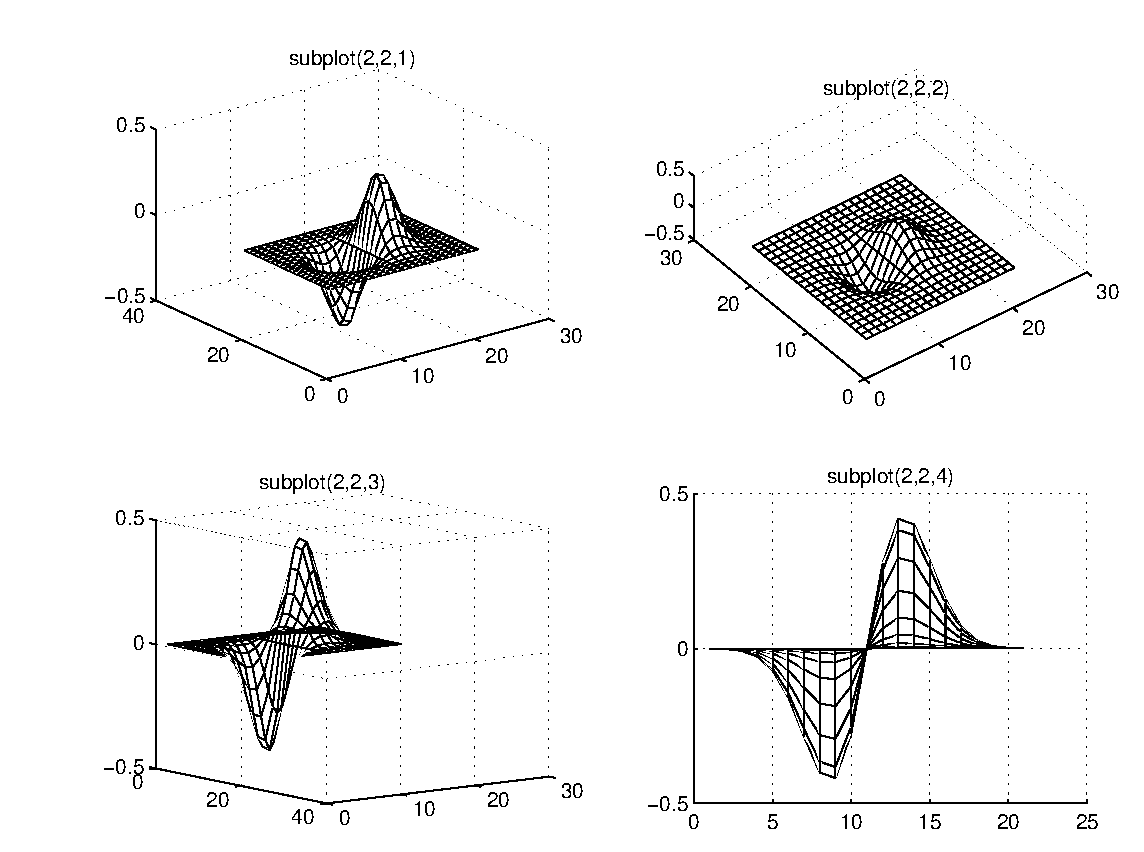
\epsfig{file=foursubplots.eps,%height=7cm ,
width=11cm, angle=0} \caption{\label{subplot}4개의 subplot:
3차원상에서 곡면의 회전}
\end{figure}

One can draw graphs with many different axes in one graphic window using {\tt subplot}. The command \texttt{\textbf{subplot(m, n, p)}} divides the current graphic window into $m \times n$ small axis, (starting from top left following the row) sets the {\tt p}-th graph as the current graph. For example, the following program makes four axes just like the picture~\ref{subplot}.

\begin{center}
\fbox{\parbox{10.5cm}{\begin{center}
\parbox{7.6cm}{\tt \% test\!$\_{}$subplot.m \\ \\
\tt [x,y] = meshgrid(-3:0.3:3, -3:0.3,3); \\
z = x.* exp(-x.\^{}2-y.\^{}2); \\
subplot(2,2,1) \\
mesh(z), title('subplot(2,2,1)') \\
subplot(2,2,2) \\
mesh(z) \\
view(-37.5, 70), title('subplot(2,2,2)') \\
subplot(2,2,3) \\
mesh(z) \\
view(-37.5, -10), title('subplot(2,2,3)') \\
subplot(2,2,4) \\
mesh(z) \\
view(0,0), title('subplot(2,2,4)')}  \end{center} }}
\end{center}
\vn The command {\tt subplot(1,1,1)} sets the graphic axis back to one.

\subsubsection{figure, clf, cla}
Command {\tt figure} produces a new figure window. \par

\begin{description}
\item[{\tt figure(N)}] \hfil\par
Produces {\tt N}-th figure window. Commands related to graphic after this will be executed in this window.
\item[{\tt clf}] \hfil\par
Everything except the window of the current figure window will be deleted. Thus, the properties of the current window will also be deleted.
\item[{\tt cla}] \hfil\par
Deletets all the lines, symbols, texts except the axis and axis markings in the current figure window.
\end{description}

\subsubsection{Inputs related to graphics}
The command \vv \texttt{\textbf{[x, y] = ginput}} \vn saves all the points that are inputted by the mouse on the current window. Cross shape is shown on the screen, and saves the points the mouse clicks. {\tt Enter} finishes this command. The command \vv \texttt{\textbf{[x, y] = ginput(n)}} \vn is exactly the same as {\tt ginput} except it only saves {\tt n} points. Use {\tt help} or {\tt doc} to earn more information..

\subsubsection{Logarithmic plot}

\begin{figure}[]
\center \epsfig{file=logarithmicplot.eps, height=7cm, %width=10cm,
angle=0} \caption{\label{log}Logarithmic plot}
\end{figure}

Command \texttt{\textbf{semilogy(x, y)}} displays the graph {\tt y} with $\log_{10}$ scale and {\tt x} with linear scale. For instance, \matlabp\texttt{\textbf{x = 0:0.01:4;}} \matlabp\texttt{\textbf{semilogy(x, exp(x)), grid}} \vn draws the graph like picture~\ref{log}. The increase of equidistant interval of {\tt y}-axis is expressed in exponent of 10. In addition, the marking in the {\tt y}-axis are drawn to show 1, 2, 3, $\ldots$, 10, 20, 30, $\ldots$, 100, $\ldots$ starting from bottom. There are also similar commands like {\tt semilogx} and {\tt loglog}. {\tt x} and {\tt y} can be vector or matrix just like they were with {\tt plot}.

\vn \textbf{Practice question:} Draw graph of $x^{2}, x^{3}, x^{4}, \exp{x^{2}}$ with $ 0\leq x \leq 10$ using {\tt semilogy}.

\subsubsection{Polar Coordinate} 

\begin{figure}[]
\center 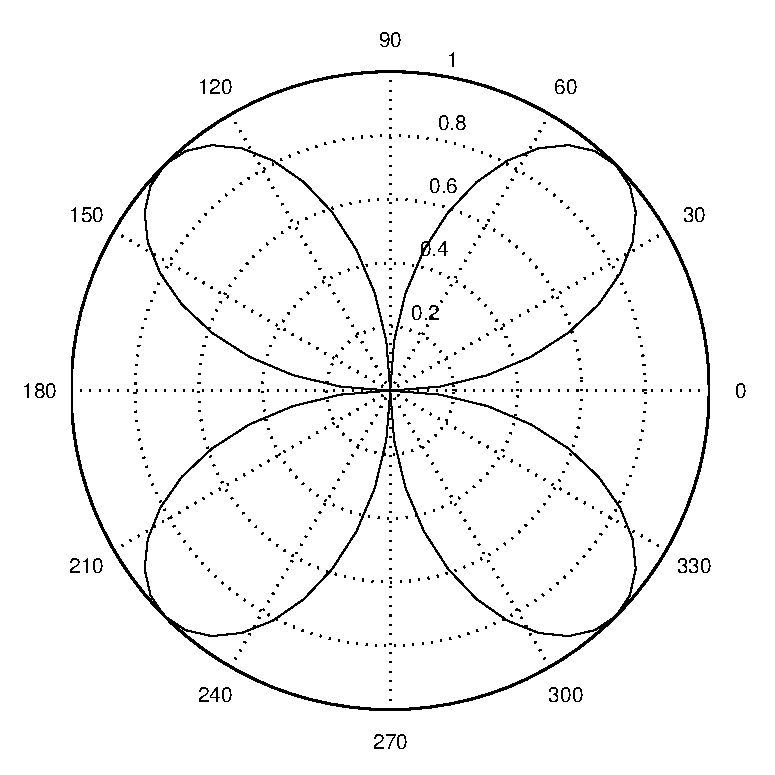
\epsfig{file=polarplot.eps,height=7cm, %width=10cm,
angle=0} \caption{Polar plot: $r=\sin 2\theta$ } \label{polar}
\end{figure}

The command \texttt{\textbf{polar(theta, r)}} uses angle $\theta$ and size $r$ to show the position of the point. For instance, \matlabp\texttt{\textbf{x = 0:pi/40:2*pi;}} \matlabp\texttt{\textbf{polar(x, sin(2*x)), grid}} \vn produces graph like picture~\ref{polar}.

\subsubsection{Drawing a Graph of a Function that Changes Quickly}

\begin{figure}
\centering
\mbox{%
\subfigure[]{%
\epsfig{file=ysina.eps,width=0.45\textwidth}} \quad
\subfigure[]{%
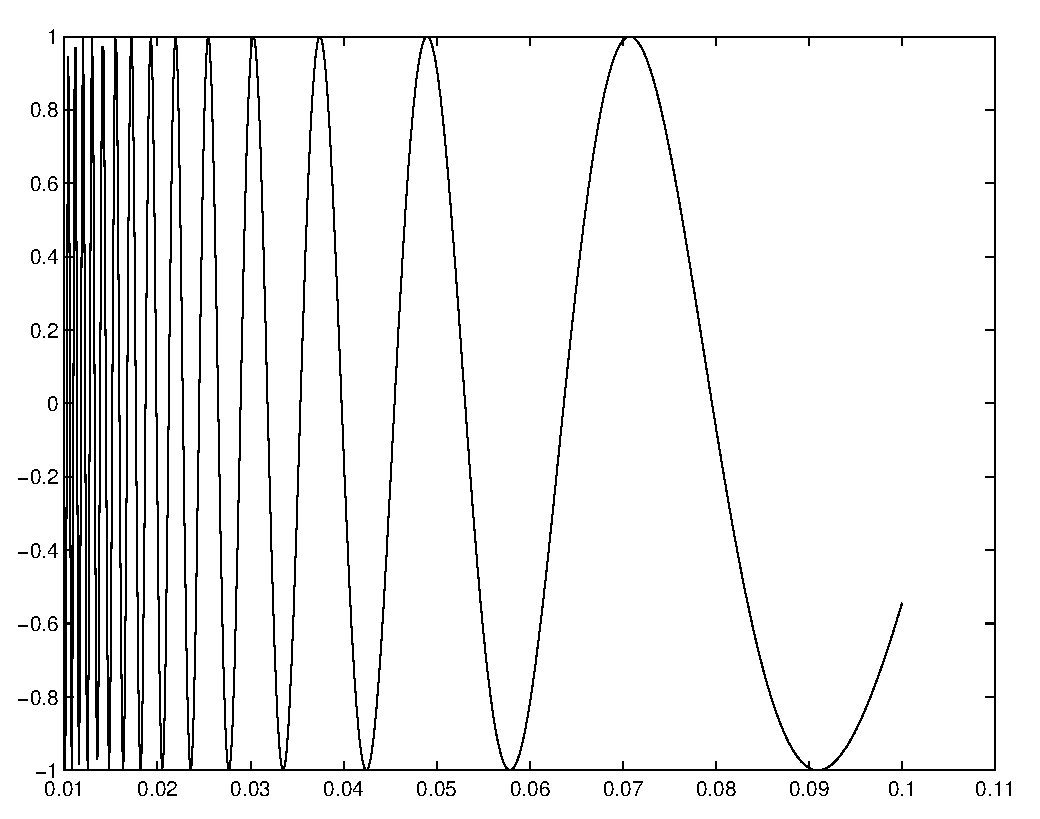
\epsfig{file=ysinb.eps,width=0.45\textwidth}}} \caption{$y
=\sin(1/x)$} \label{sin}
\end{figure}

Until now, the graphs were drawn with data that has $x$-axis all distributed equally, like the example \texttt{\textbf{x = 0:0.01:4}}. If a function to be drawn rapidly changes in a certain domain, then the distribution of $x$-axis will be inefficient, and the graph will not be drawn properly. For instance, \matlabp\texttt{\textbf{x = 0.01:0.001:0.1;}} \matlabp\texttt{\textbf{plot(x, sin(1./x))}} \vn will draw the graph like picture~\ref{sin}(a). However, if the increment of $x$ is reduced to 0.0001, then the graph like picture~\ref{sin}(b) will be drawn. The two graphs are clearly different in the domain $x < 0.04$.

\vv Matlab provides {\tt fplot}, which is a more efficient function. When it comes to drawing a function like $\sin(1/x)$, {\tt fplot} calculates rapid changing places more frequently. However, the command {\tt fplot} has a demerit, which is it must use function file.

\subsubsection{Many Commands related to 2 Dimensional Graphs}
Matlab provides many commands that express functions into graphs. Here, we state some examples, but we wish for the reader to use {\tt help} or {\tt doc} to get more detailed information.

\begin{description}
\item[\tt bar] \hfil\par Draws bar graph. \item[\tt compass] \hfil\par Displays the vector with entries size and direction of complex number with an arrow starting from the origin.
\item[\tt errorbar] \hfil\par Displays error bar. \item[\tt hist] \hfil\par Draws histogram. \item[\tt quiver] \hfil\par Draws many different types of vector fields(for instance, gradient) using little arrows.
\item[\tt fill] \hfil\par Draws polygon and fills in with given color.
\end{description}

\subsection{3 Dimensional Graph}
Matlab provides many functions that can express 3 dimensional graphs. This susbsection will be a brief introduction to these functions.

\subsubsection{Plot3}

\begin{figure}
\centering
\mbox{%
\subfigure[]{%
\epsfig{file=plot3a.eps,width=0.45\textwidth}} \quad
\subfigure[]{%
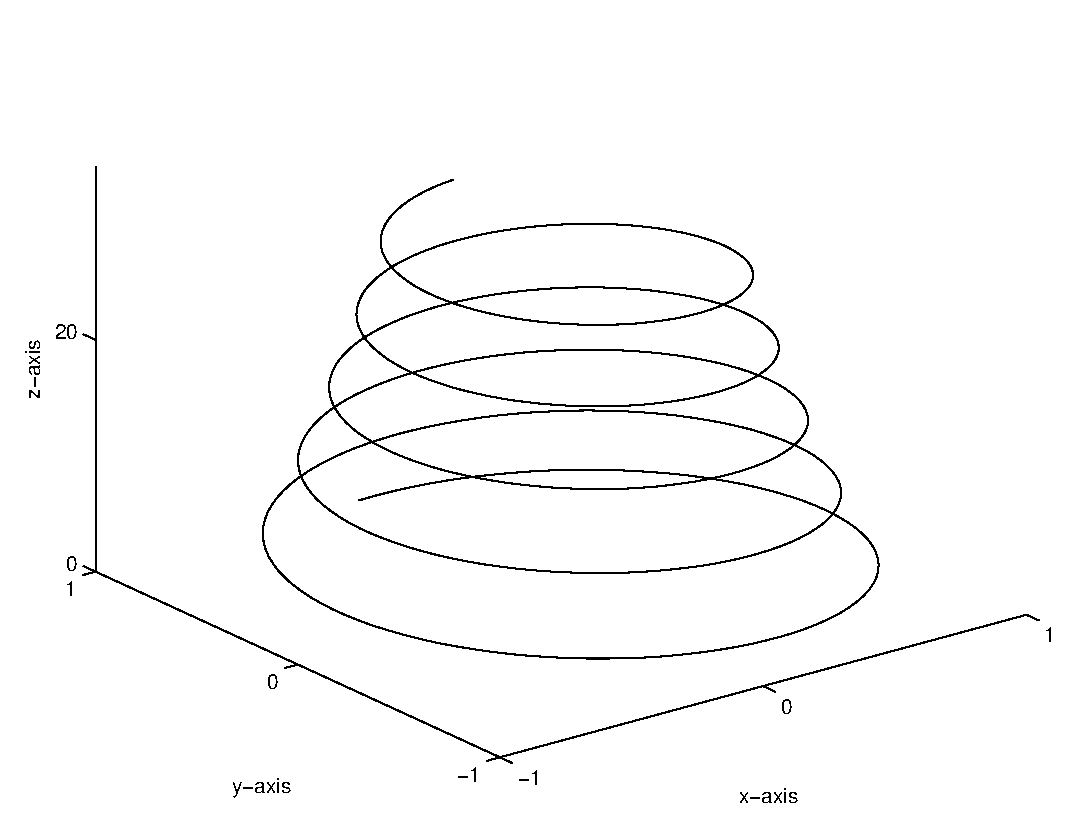
\epsfig{file=exampleofplot3b.eps,width=0.45\textwidth}}} \quad
\caption{example of command plot3}\label{plot3}
\end{figure}

The command {\tt plot3} is a 3 dimensional version of {\tt plot}, and if we write \matlabp\texttt{\textbf{plot3(x, y, z)}} \vn then a line connecting the points $(x_i, y_i, z_i)$ will be drawn in 3 dimension. For instance, \matlabp\texttt{\textbf{plot3(rand(1,10), rand(1,10), rand(1,10))}} \vn uses 10 random points to draw a line in 3 dimension, like picture~\ref{plot3}(a). And another example, \matlabp\texttt{\textbf{t = 0:pi/50:10*pi;}} \matlabp\texttt{\textbf{plot3(exp(-0.02*t).*sin(t), exp(-0.02*t).*cos(t), t), \ldots}} \par\texttt{\textbf{xlabel('x-axis'), ylabel('y-axis'), zlabel('z-axis') }}\vn draws a dwindling spiral like picture~\ref{plot3}(b). Be careful on the direction of $x$-axis, $y$-axis, $z$-axis, and pay attention to the fact that label was marked for each axis.

\subsubsection{Mesh Surface}
The following is an example regarding mesh surface.

\begin{center}
\fbox{\parbox{10.5cm}{\begin{center}
\parbox{8.4cm}{\tt \% Mexican\!$\_{}$hat.m \\ \\
\tt [x y] = meshgrid(-7.5:0.5:7.5, -7.5:0.5:7.5);  \\
r = sqrt(x.\^{}2 + y.\^{}2) + eps; \\
z = sin(r)./r; \\
mesh(z);}  \end{center} }}
\end{center}

\vv To know how these surfaces are drawn, let us study a simple example like $z = x^{2} - y^{2}$. We want a graph that shows the change in $z$ value when there is a change in values in $x$-$y$ plane. Let us think only in the domain $0 \leq x \leq 5, 0 \leq y \leq 5$ for this example. First use Matlab command {\tt meshgrid} to produce grid on the $x$-$y$ plane where the surface will be drawn. \matlabp\texttt{\textbf{[x y] = meshgrid(0:5, 0:5)}} \vn This command produces two matrices {\tt x, y} like the following.
$$\begin{array}{ccccccc}
{\tt x =} & & & & & & \\
& 0 & 1 & 2 & 3 & 4 & 5 \\
& 0 & 1 & 2 & 3 & 4 & 5 \\
& 0 & 1 & 2 & 3 & 4 & 5 \\
& 0 & 1 & 2 & 3 & 4 & 5 \\
& 0 & 1 & 2 & 3 & 4 & 5 \\
& 0 & 1 & 2 & 3 & 4 & 5
      \end{array}\qquad\qquad
\begin{array}{ccccccc}
{\tt y =} & & & & & & \\
& 0 & 0 & 0 & 0 & 0 & 0 \\
& 1 & 1 & 1 & 1 & 1 & 1 \\
& 2 & 2 & 2 & 2 & 2 & 2 \\
& 3 & 3 & 3 & 3 & 3 & 3 \\
& 4 & 4 & 4 & 4 & 4 & 4 \\
& 5 & 5 & 5 & 5 & 5 & 5
\end{array}$$

\vn As we can see from above, matrix {\tt x} represents each grid of $x$-axis, and matrix {\tt y} represents each grid of $y$-axis. If the grid of $x$-direction and that of $y$-direction are of same shape, then we can write in the following short form. \matlabp\texttt{\textbf{[x y] = meshgrid(0:5)}} \vn And as can be predicted with the Matlab matrix operation, the command \texttt{\textbf{z = x.\^{}2-y.\^{}2}} produces the following matrix.
$$\begin{array}{rrrrrrr}
{\tt z =} & & & & & & \\
& 0  &  1  &  4  &  9  &  16  &  25 \\
& -1  &  0  &  3  &  8  &  15  &  24 \\
& -4  &  -3  &  0  &  5  &  12  &  21 \\
& -9  &  -8  &  -5  &  0  &  7  &  16 \\
& -16  &  -15  &  -12  &  -7  &  0  &  9 \\
& -25  &  -24  &  -21  &  -16  &  -9  &  0
\end{array}$$

\vn For instance, at the point $(5, 2)$, z takes the value $5^{2}-2^{2} = 21$. Fortunately, one does not need to be concerned with the precise relationship between the coordinate system of the grid and the index of the matrix. This is automatically adjusted by {\tt meshgrid}.

\begin{figure}[]
\center 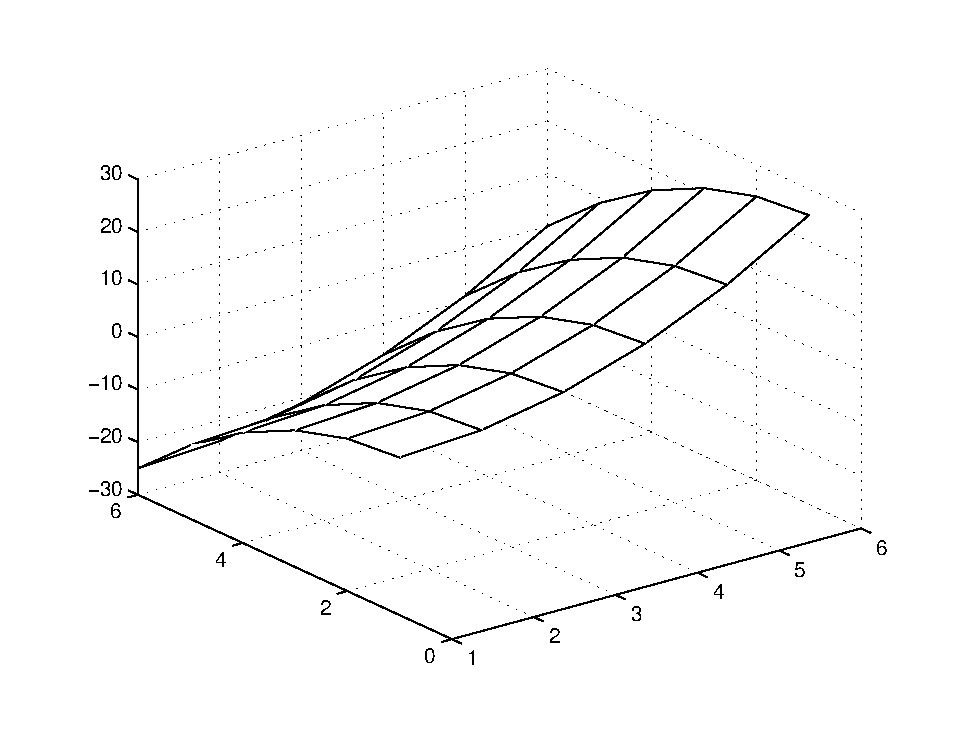
\epsfig{file=surface.eps, %fig7surf.eps,
height=7cm,%width=10cm,
angle=0} \caption{curved surface $z = x^{2}-y^{2}$} \label{surf}
\end{figure}

\vv The command {\tt mesh(z)} produces graph with lattice-like surface, where the points on the grid are raised to the surface and then connected to form the lattice. In other words, {\tt mesh} draws a `wire mesh'-like surface. If one does not want color, then one can type \matlabp{\tt mesh(z,'EdgeColor','black')} \vn In addition, another command {\tt surf} draws a lattice-like surface composed of small colored tiles. Use {\tt help} or {\tt doc} to learn more about {\tt mesh} and {\tt surf}.

If one is using Matlab student edition, then one must know that there is a limit to grid size when using {\tt meshgrid}. The limit is that the size of the row or column of matrix must be at most 32, and the size of matrix must not exceed 8192.

\vn \textbf{Practice question:} Use the command  \vv \texttt{\textbf{[x y] = meshgrid(0:0.25:5);}} \vn to draw a denser mesh than picture~\ref{surf}.

\vn \textbf{Practice question:} The distribution of temperature on the iron plate is as follows.
$$u(x, y) = 80 y^{2} e^{-x^{2}-0.3y^{2}}$$ \noindent With the domain $-2.1 \leq x \leq 2.1, -6 \leq y \leq 6$, draw the curved surface $u$ with the grid size of each direction as 0.15.

\subsubsection{Drawing Contour}
\begin{figure}
\centering
\mbox{%
\subfigure[]{%
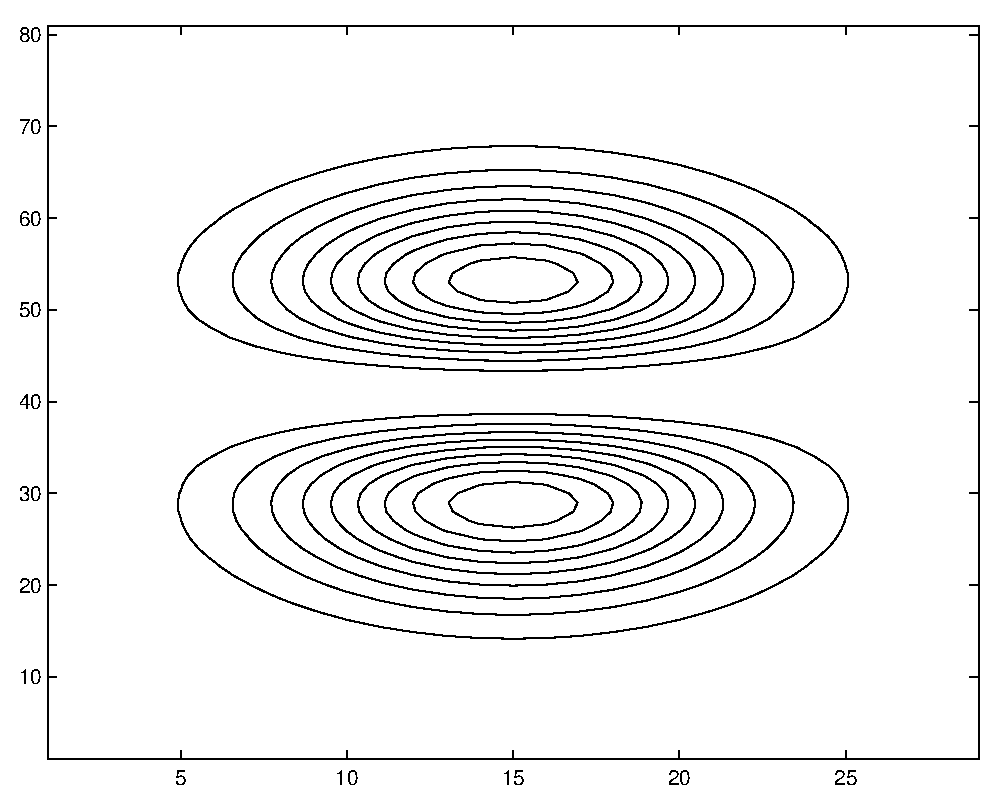
\epsfig{file=contoura.eps,width=0.45\textwidth}} \quad
\subfigure[]{%
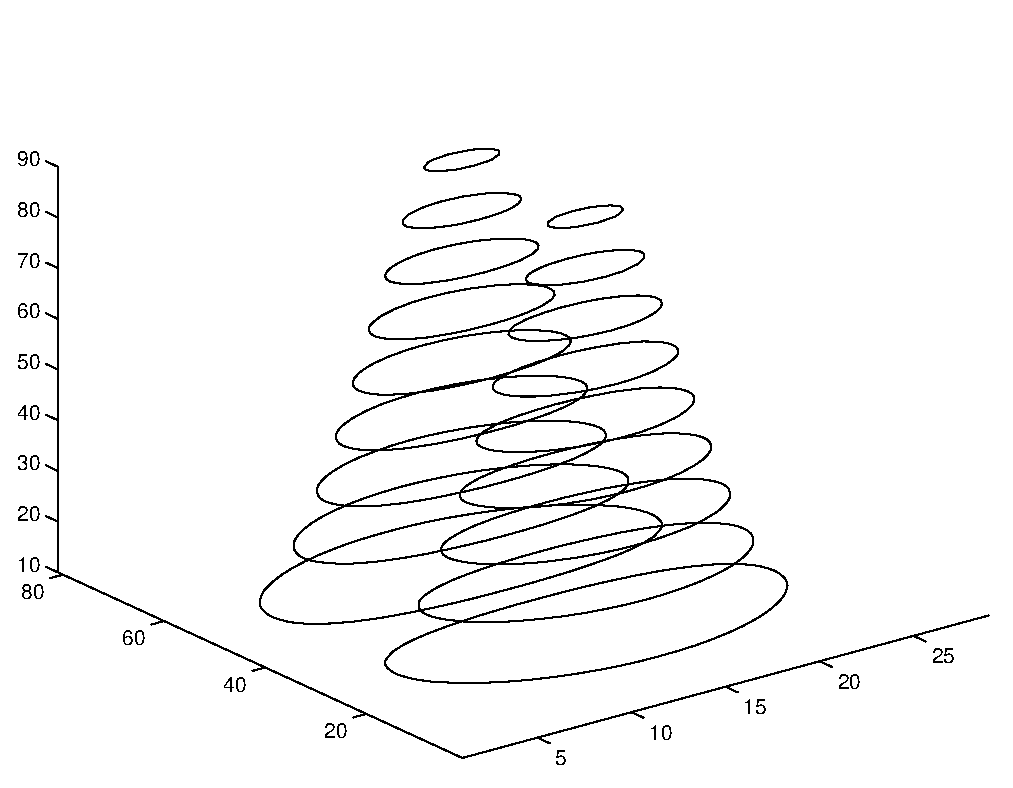
\epsfig{file=contour3b.eps,width=0.45\textwidth}}} \caption{Contour
plot} \label{contour}
\end{figure}

After solving the practice questions above, execute the following command. \matlabp\texttt{\textbf{ contour(u)}} \vn Then, one can earn a contour(isothermal line) about the distribution of temperature like picture~\ref{contour}(a). The command {\tt contour} can take second input variable. For this second variable, one inputs how many lines the contour will draw or a vector with specific values for drawing contour. Use command {\tt contour3} to draw a 3 dimensional contour like picture~\ref{contour}(b). One can make contour label with the command {\tt clabel}.

\begin{figure}
\centering
\mbox{%
\subfigure[]{%
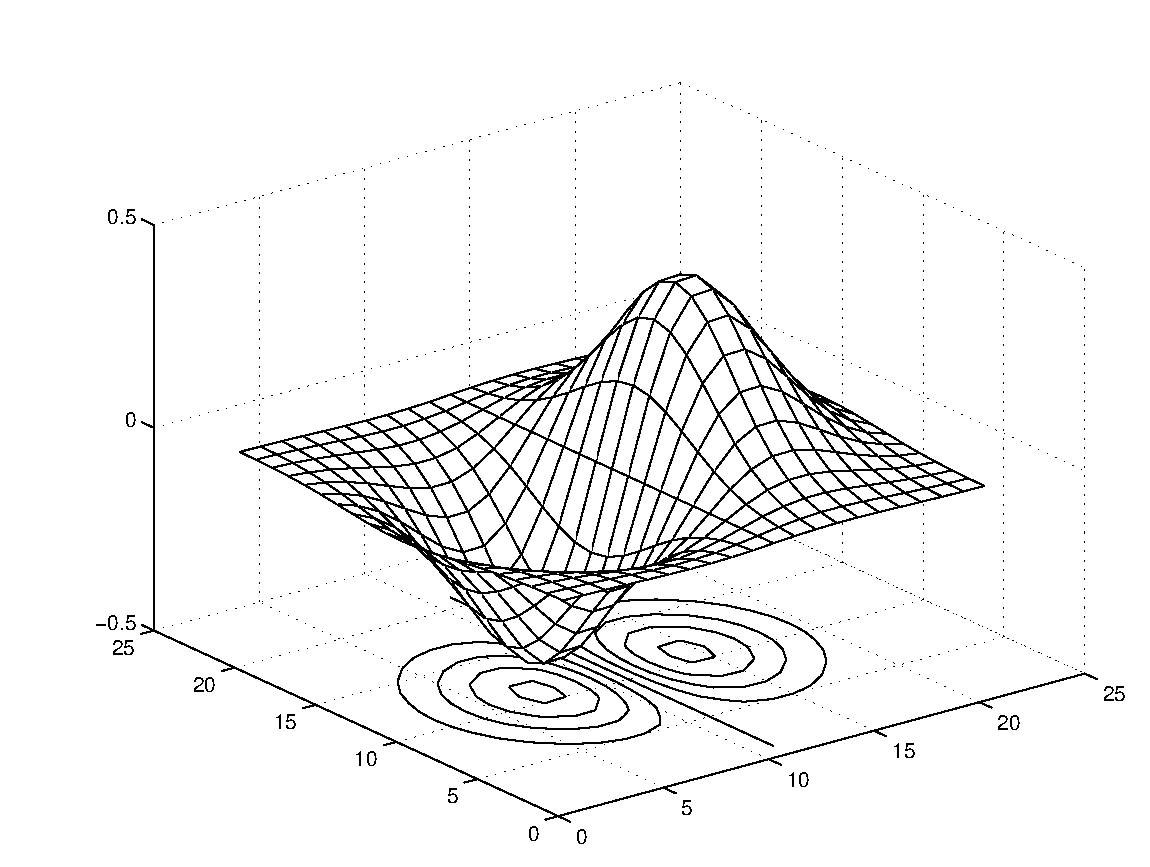
\epsfig{file=fig710a.eps,width=0.45\textwidth}} \quad
\subfigure[]{%
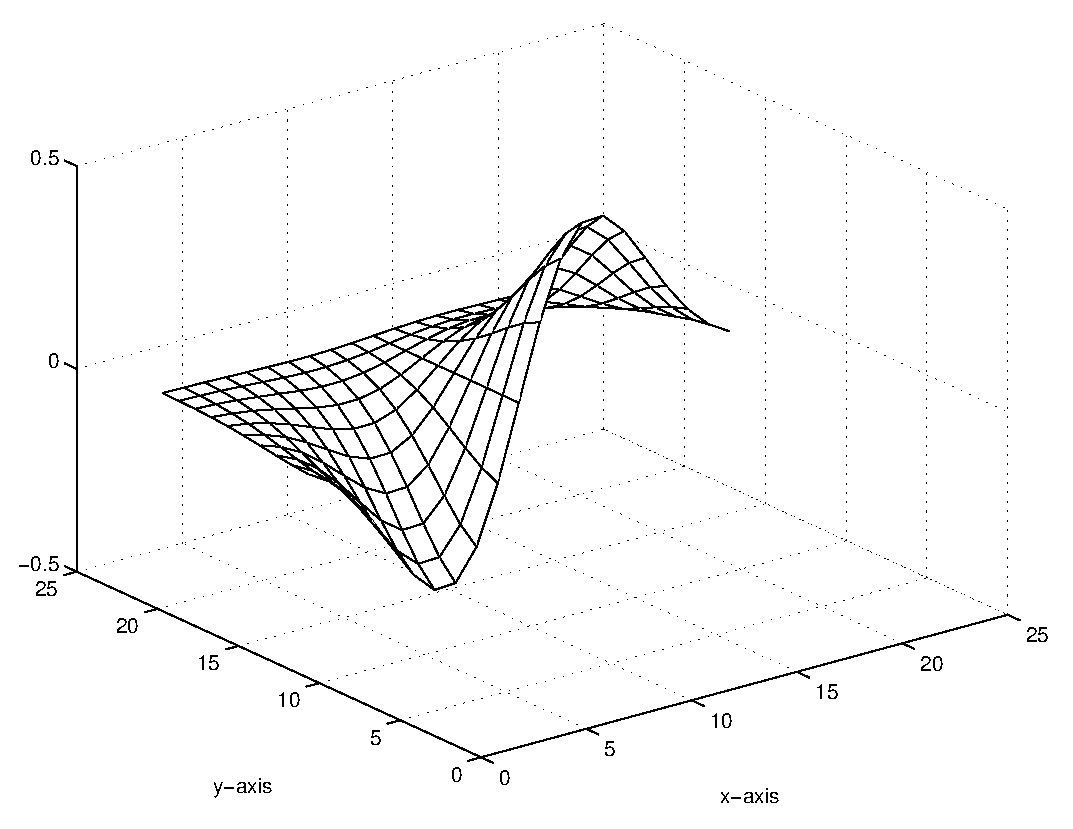
\epsfig{file=fig710b.eps,width=0.45\textwidth}}} \caption{(a)
meshc \quad (b) Erasing part of curved surface} \label{meshc}
\end{figure}

\vv To display both contour and mesh together, one can use {\tt meshc} or {\tt surfc}. For instance, the following program \matlabp\texttt{\textbf{[x y] = meshgrid(-2:0.2:2); }} \matlabp\texttt{\textbf{ z = x.*exp(-x.\^{}2 - y.\^{}2); }} \matlabp\texttt{\textbf{meshc(z);}} \vn draws a graph like picture~\ref{meshc}(a).

\subsubsection{Deletion of Curved Surface Due to NaN(Not a Number)}
If the matrix that holds information on the curved surface contains NaN, then this value does not appear in the graph, and because of this, a part of the curved surface will be omitted. Let us study the following example.

\begin{center}
\fbox{\parbox{10.5cm}{\begin{center}
\parbox{8.0cm}{\tt \% cropping.m \\ \\
\tt [x y] = meshgrid(-2:.2:2);  \\
z = x.*exp(-x.\^{}2 - y.\^{}2); \\
c = z;\qquad \% preserve the original surface \\
c(1:11, 1:21) = nan; \\
mesh(c), xlabel(`x-axis'), ylabel(`y-axis')}  \end{center} }}
\end{center}
\vn The above program will display the graph like picture~\ref{meshc}(b).

\subsubsection{quiver}
The command {\tt quiver} draws a vector that starts at 2 dimensional point. Although it is drawn in 2 dimensional graph, it is occasionally used with {\tt contour}, which helps understanding changes in 3 dimensional curved surfaces. For instance, let us think about $V = x^{2} + y$, which is a scalar function with 2 variables for input. The gradient of V is defined as the following vector field.
\begin{eqnarray*}
\nabla V & = & \left(\frac{\partial V}{\partial x}, \frac{\partial
V}{\partial y}\right) \\
         & = & (2x, 1)
\end{eqnarray*}

\begin{figure}[]
\center 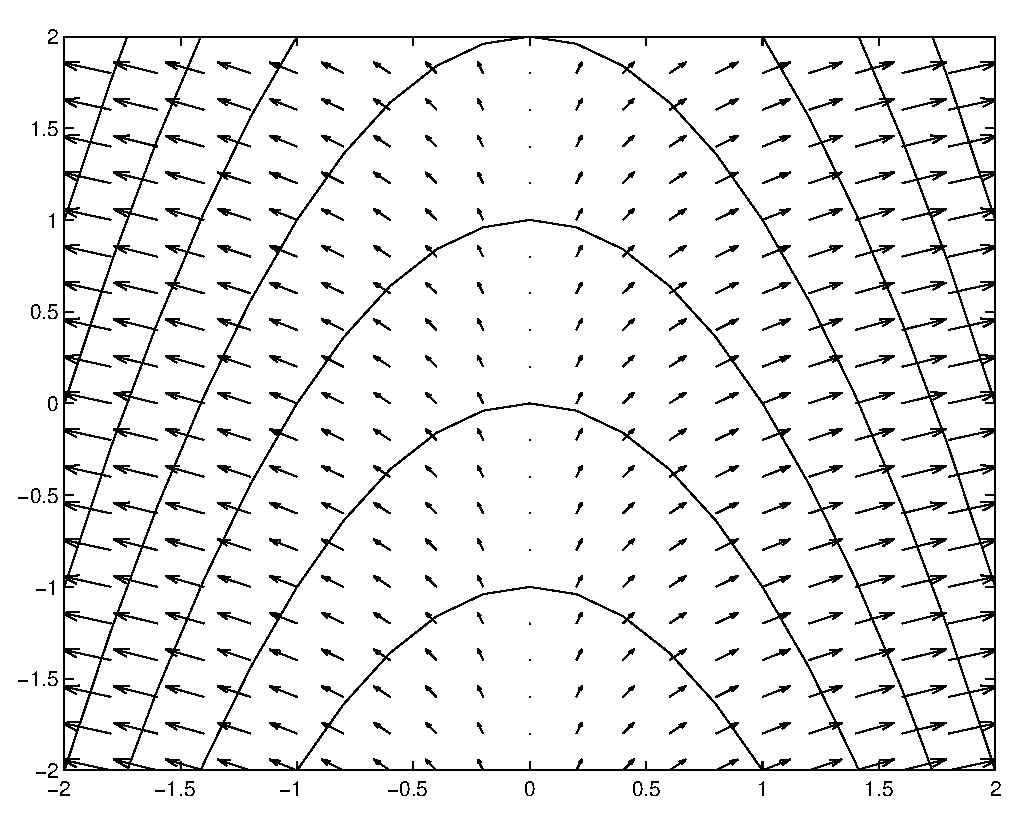
\epsfig{file=fig711.eps,height=7cm, %width=10cm,
angle=0} \caption{Gradient and contour} \label{grad}
\end{figure}

\noindent The following program draws the direction of $\nabla V$ for each points in $x$-$y$ plane(refer to picture~\ref{grad}).

\begin{center}
\fbox{\parbox{10.5cm}{\begin{center}
\parbox{5.6cm}{\tt \% test\!$\_{}$quiver.m \\ \\
\tt [x y] = meshgrid(-2:.2:2);  \\
V = x.\^{}2 + y; \\
dx = 2*x; \\
dy = ones(size(y)); \\
axis equal \\
contour(x, y, V), hold on \\
quiver(x, y, dx, dy), hold off}  \end{center} }}
\end{center}

`Contour' is a series of {\tt level surface}. Gradient of a random point is perpendicular to the level surface that passes through that point. When drawing a contour, the vectors {\tt x} and {\tt y} are required for labeling the axes. What will happen if take this out and just use {\tt contour(V)} and execute the above {\tt test\!$\_{}$quiver.m}? Let us try to predict the result before we execute it.

Another option regarding {\tt quiver} is that one can change the size of the arrows. See {\tt help} or {\tt doc}.

If it is not possible to differentiate the vector $V$ or if one does not wish to differentiate it, then one can use the command {\tt gradient} to calculate the derivative.
\matlabp\texttt{\textbf{[dx dy] = gradient(V, 0.2, 0.2);}} \vn 0.2 means the increment with respect to $x$ and $y$ directions for approximate calculation.

\subsubsection{Pseudocolor}
The following program  \matlabp\texttt{\textbf{[x, y] = meshgrid(-2:.2:2); }} \matlabp\texttt{\textbf{z = x.*exp(-x.\^{}2 - y.\^{}2); }} \matlabp\texttt{\textbf{pcolor(z), shading flat, colormap(hot) }} \vn draws a contour that expresses height using mixture of red, orange, and yellow. The command {\tt shading flat} eliminates the grid line. {\tt pcolor} means pseudocolor. Each element of the matrix {\tt z} is used as index of color map(in this case hot) that determines the color which will express the element. If one wants a cool color, then try {\tt colormap(cool)}.\^{}\^{} Does it feel cool? There is yet another color map, {\tt colormap(hsv)}, where {\tt hsv} stands for huge-saturation-value.

\subsubsection{Visualization of matrix}

\begin{figure}[]
\center 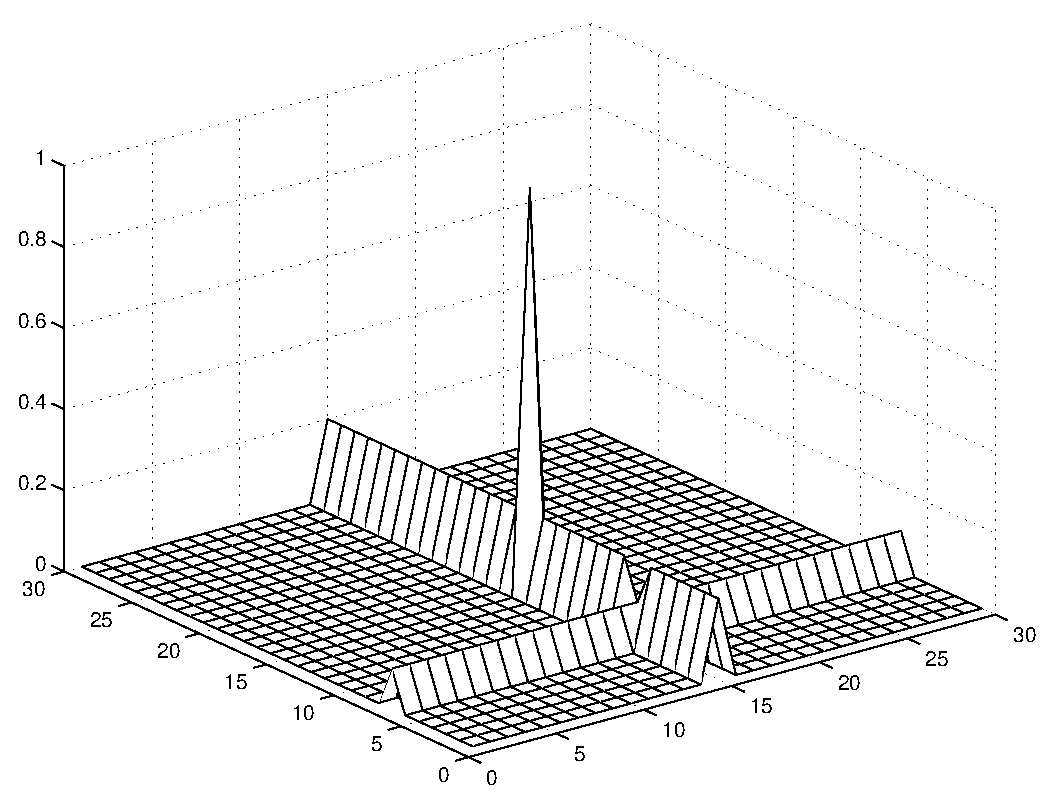
\epsfig{file=viewmat.eps,height=7cm,%width=10cm,
angle=0} \caption{visualization of matrix} \label{mat}
\end{figure}

The command {\tt mesh} can `visualize' the matrix. The following program displays the graph like picture~\ref{mat}.

\begin{center}
\fbox{\parbox{10.5cm}{\begin{center}
\parbox{4.7cm}{\tt \% visual\!$\_{}$mat.m \\ \\
\tt a = zeros(30);  \\
a(:,15) = 0.2*ones(30,1); \\
a(7,:) = 0.1*ones(1,30); \\
a(15,15) = 1; \\
mesh(a)}  \end{center} }}
\end{center}
\vn The size of the matrix {\tt a} is $30 \times 30$. The middle element {\tt a(15,15)} is 1, and every element of the 7-th row is 0.1, and the remaining elements of the 15-th row is 0.2. {\tt mesh(a)} cognizes every rows and columns of matrix a as coordinates of $x$-$y$. In other words, the value of {\tt a(i,j)} is the height of the curved surface mesh at point {\tt (i,j)}.

\subsubsection{Rotating 3 Dimensional Graph}
{\tt view} is a command which designates observation point when viewing a 3 dimensional graph. To see how this works, let us execute the following program which rotates the visualized matrix picture~\ref{mat}.

\begin{center}
\fbox{\parbox{10.5cm}{\begin{center}
\parbox{5cm}{\tt \% rotation.m \\ \\
\tt a = zeros(30);  \\
a(:,15) = 0.2*ones(30,1); \\
a(7,:) = 0.1*ones(1,30); \\
a(15,15) = 1; \\
el = 30; \\
for az = -37.5:15:-37.5+360 \\
\phantom{for}mesh(a), view(az, el) \\
\phantom{for}pause(0.5) \\
end}  \end{center} }}
\end{center}
\vn The command {\tt view} requires two angles. The first, as can be seen in the example, is azimuth {\tt az} on the $x$-$y$ plane that has degree as its unit. {\tt az} rotates the observation point about $z$-axis - in other words, the 'sharp point' at $(15,15)$ in picture~\ref{mat} - counterclockwise. The default value for {\tt az} is $-37.5^{\circ}$. Therefore, the above program rotates the observation point about $z$-axis $15^{\circ}$ each time from the default value. The second angle of {\tt view} is {\tt el} which expresses altitude with degree as its unit. This means the angle between the $z$-axis and $x$-$y$ plane. For instance, $90^{\circ}$ represents 2 dimensional graphic, in other words, looking down from above. If the value of altitude is positive, then the observer is above the $x$-$y$ plane, and if negative, then is below the plane. The default value is $30^{\circ}$.

\vv The command {\tt pause(n)} stops the execution for {\tt n} seconds.

\vn \textbf{Practice question:} Fix the above program so that the value of {\tt az} is fixed as the default value and and the value of {\tt el} is gradually changing.

\subsubsection{Lighting}
One can materialize lighting and shadow effect using the command {\tt surfl}. Try the following.

\matlabp\texttt{\textbf{[x, y] = meshgrid(-2:0.05:2);}}
\matlabp\texttt{\textbf{z = x.*exp(-x.\^{}2 - y.\^{}2); }}
\matlabp\texttt{\textbf{surfl(z, [-20 50]), colormap(gray),
shading flat}} \vn The location of the source of light is determined by the second variable of {\tt surfl}, with the first value being azimuth and the second being altitude. To make a natural reflection light, one must set the grid compact so that the grid is not visualizable. (In this case, $81\times 81$)